\section{Introduction}

\begin{frame}
	\frametitle{What is a PID controller?}
	\begin{definition}
		A \textbf{P}roportional \textbf{I}ntegral \textbf{D}eriviative controller is a loop feedback controller with continious time equation:
		\begin{equation*}
			u(t) = 	\underbrace{\vphantom{\int^t_0e(\tau)d\tau}K_p e(t)}_\text{Proportional Action} 
					+ \underbrace{K_i\int^t_0e(\tau)d\tau}_\text{Integral Action} 
					+ \underbrace{\vphantom{\int^t_0e(\tau)d\tau} K_d \frac{de(t)}{dt}}_\text{Derivative Action}
		\end{equation*}
		\begin{figure}
			\centering
			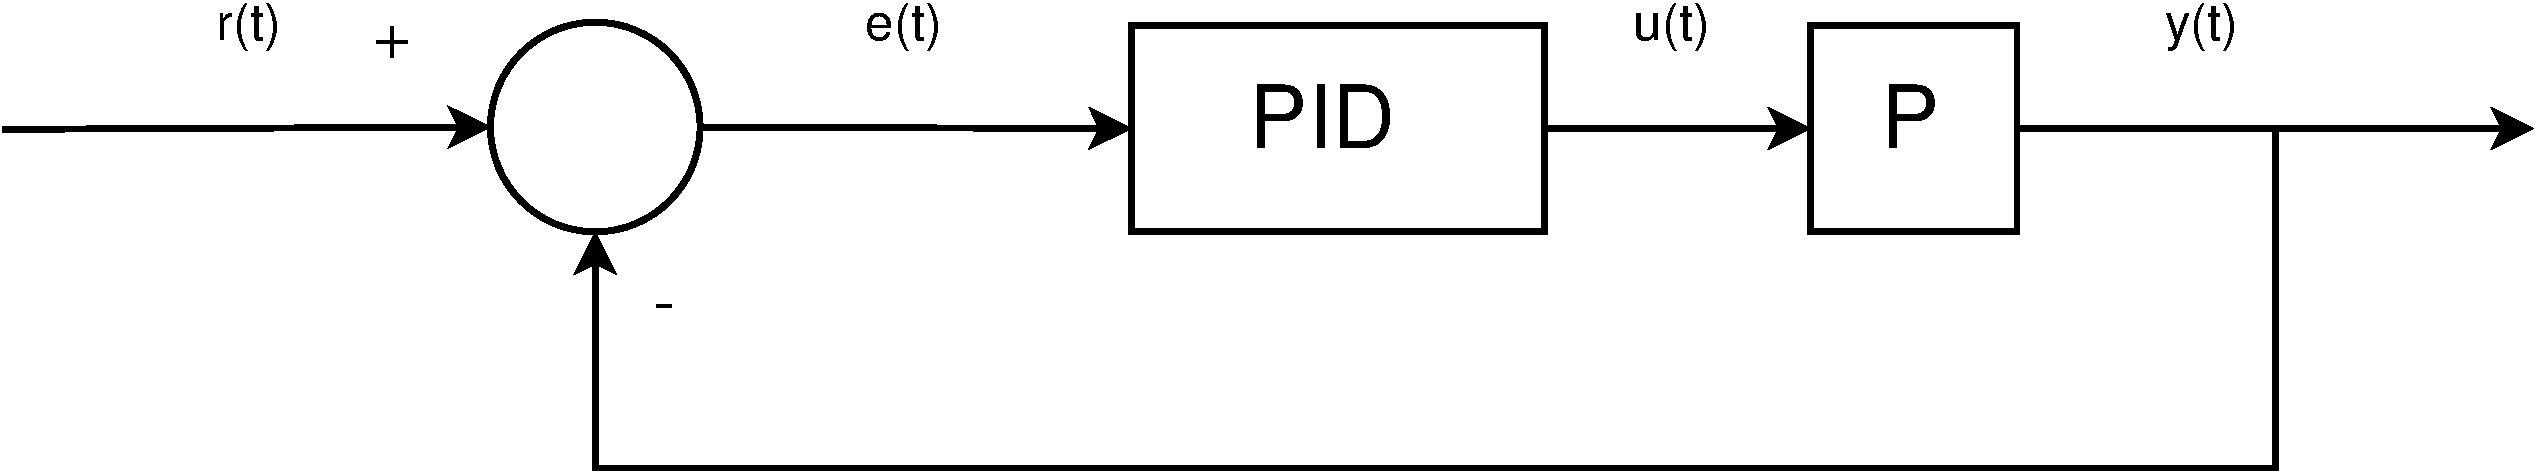
\includegraphics[width=0.8\linewidth]{img/PID}
		\end{figure}
	\end{definition}
	More than 90\% of all closed loop controllers are PID
\end{frame}

\begin{frame}
\frametitle{What is a PID controller?}
Content of the second slide
\end{frame}
